\documentclass{article}
\usepackage[utf8]{inputenc}
\usepackage{graphicx}
\graphicspath{ {./images/} }
\usepackage{amsmath}
\usepackage{hyperref}
%\usepackage[english]{babel}
\usepackage{pdfpages}

\usepackage{chemfig}

\usepackage[left=2cm,right=1cm, top=2cm,bottom=2cm,bindingoffset=0cm]{geometry}
\renewcommand{\normalsize}{\fontsize{14}{18pt}\selectfont}
\newcommand{\specialcell}[2][c]{%
	\begin{tabular}[#1]{@{}c@{}}#2\end{tabular}}
\renewcommand{\normalsize}{\fontsize{14}{18pt}\selectfont}

\title{Studying  fermentation via RNA-seq  }
\author{ Ignat Sonets, Kamilla Faizullina}
\date{\empty}

\begin{document}
	
		\catcode`\_=\active
	\catcode`\^=\active
	
\maketitle
 
 
\section{Introduction}
 
 Hello! Today we perform differential expression analysis for RNA-seq data of S.cerevisiae to estimate changes in gene expression levels while baking the bread. But before we start, I want to briefly introduce some data about yeasts and fermentation process.
 As we all  know, for making bread we use yeasts. Yeasts eat sugars and put dough to rise. But what processes occur? First, it is an anaerobic process. You might be surprised, but yeasts undergo ethanol fermentation during dough rising (and if you make your dough with more water and leave your mixture near a heat source for about 2-3 days, you will recreate the ancient beer recipe, as it was done by ancient Egyptians.). Fermentation of sugars in flour is the core of bread making. How fermentation works? Ethanol fermentation transforms one mole of glucose into two moles of ethanol and two moles of carbon dioxide (which is the most important component for bread making), producing two moles of ATP (unfortunately, it won't make bread a Red Bull) in the process. 
 Details about given process are taken from \cite{1}.
 The overall chemical formula for alcoholic fermentation is:
 
 \chemfig{C6H12O6  $\rightarrow$ 2 C2H5OH + 2 CO2}
 
 Sucrose is a sugar composed of a glucose linked to a fructose. In the first step of alcoholic fermentation, the enzyme invertase cleaves the glycosidic linkage between the glucose and fructose molecules.(NB: almost the same process can be made with saccharose, which is also dimer consist of glucose and fructose, but with different glycoside bond).
 
 \ce{C12H22O11 + H2O + invertase → 2 C6H12O6}
 
 Next, each glucose molecule is broken down into two pyruvate molecules in a process known as glycolysis \cite{2}. Glycolysis is summarized by the equation:
 
 C6H12O6 + 2 ADP + 2 Pi + 2 NAD+ → 2 CH3COCOO− + 2 ATP + 2 NADH \\
 + 2 H2O + 2 H+
 
 CH3COCOO− is pyruvate, and Pi is inorganic phosphate. Finally, pyruvate is converted to ethanol and CO2 in two steps, regenerating oxidized NAD+ needed for glycolysis:
 
 1. CH3COCOO− + H+ → CH3CHO + CO2
 
 catalyzed by pyruvate decarboxylase
 
 2. CH3CHO + NADH + H+ → C2H5OH + NAD+
 
 This reaction is catalyzed by alcohol dehydrogenase.
 So, we think, that yeasts would behave differently between 2 states: before the start of the fermentation and during the fermentation, because cells will(and should) respond to its changing environment. To provide necessary enzymes for fermentation, the yeast cell should start their synthesis (i.e. translation). To start their synthesis, transcription (DNA to RNA information transfer) should begin. So your gene expression(i.e. the process by which information from a gene is used in the synthesis of a functional gene product that enables it to produce protein as the end product\cite{3}) changes. But how to e s t i m a t e this? Differential expression analysis at your service. To do this, we need RNA-seq data, reference genome of S.cerevisiae, annotation file (to find which gene changed its expression levels) and skills. By measuring differences in gene expression we can not only confirm our suggestions, but also discover new data that could potentially be useful in biotechnology(i.e. modifying enzymes, maybe adding new enzymes or even massive genomic rearrangements) and even on your kitchen by, for example, tweaking flour/water proportions, changing flour type, adding more sugar etc. This could be done with tries and errors and many repeats, but if we can obtain some evidence-based discoveries, why not?
 Let's get started.
 
 
 \section{Data}
In order to study RNA expression levels, we use RNA-seq data from yeast obtained before and during fermentation \cite{data}. We also use Saccharomyces cerevisiae assembly R64  strain S288C from NCBI \cite{ncb} as a reference genome data. This is a species of yeast. 


\section{Methods}
 RNA-seq differential gene expression analysis allows to measure  quantitative changes in the expression levels between the experiments.  We analyze yeast data before and during fermentation as we would like to compare expression of  different genes between  fermentation process and normal growth. 
 
 First, we should make alignment. We use HISAT2 which allows us make  alignment  for RNA sequencing reads \cite{hisat}. The utility DESeq2 is used to perform differential gene expression analysis \cite{deseq}. This method is based on using negative binomial distribution in the model. We use command $\textrm{featureCounts}$ from the Subread package \cite{featurecounts} for counting reads and command $\textrm{gffread}$ \cite{gff} to prepare results for DESeq2. 
 
 After using DESeq2, we have output results. To make interpretation of results, we use Saccharomyces Genome Database  by Stanford \cite{ontology}. 
 
 
%\newpage 
%\newpage 
\begin{thebibliography}{9}
	\bibitem{1} https://en.wikipedia.org/wiki/Ethanol_fermentation#Biochemical_process_of_fermentation_of_sucrose



	\bibitem{2}	
	Stryer, Lubert (1975). Biochemistry. W. H. Freeman and Company. ISBN 978-0-7167-0174-3.
	
		\bibitem{3}
		https://en.wikipedia.org/wiki/Gene_expression
	
	
 \bibitem{data}

ftp.sra.ebi.ac.uk/vol1/fastq/SRR941/SRR941816/SRR941816.fastq.gz 

ftp.sra.ebi.ac.uk/vol1/fastq/SRR941/SRR941817/SRR941817.fastq.gz 

 ftp.sra.ebi.ac.uk/vol1/fastq/SRR941/SRR941818/SRR941818.fastq.gz 
 
 ftp.sra.ebi.ac.uk/vol1/fastq/SRR941/SRR941819/SRR941819.fastq.gz (282 Mb)

 \bibitem{ncb}
 Sayers EW, Agarwala R, Bolton EE, Brister JR, Canese K, Clark K, Connor R, Fiorini N, Funk K, Hefferon T, Holmes JB, Kim S, Kimchi A, Kitts PA, Lathrop S, Lu Z, Madden TL, Marchler-Bauer A, Phan L, Schneider VA, Schoch CL, Pruitt KD, Ostell J. Database resources of the National Center for Biotechnology Information. Nucleic Acids Res. 2019 Jan 8;47(D1):D23-D28. doi: 10.1093/nar/gky1069. PubMed PMID: 30395293; PubMed Central PMCID: PMC6323993. 2: Sayers EW, Cavanaugh M, Clark K, Ostell J, Pruitt KD, Karsch-Mizrachi I. GenBank. Nucleic Acids Res. 2019 Jan 8;47(D1):D94-D99. doi: 10.1093/nar/gky989. PubMed PMID: 30365038; PubMed Central PMCID: PMC6323954.
 
 
 
\bibitem{hisat}
Kim D, Langmead B and Salzberg SL. HISAT: a fast spliced aligner with low memory requirements. Nature Methods 2015

\bibitem{deseq}
Love MI, Huber W, Anders S (2014). “Moderated estimation of fold change and dispersion for RNA-seq data with DESeq2.” Genome Biology, 15, 550. doi: 10.1186/s13059-014-0550-8. 


\bibitem{featurecounts}
Liao Y, Smyth GK and Shi W (2014).  featureCounts:  an efficient general pur-pose program for assigning sequence reads to genomic features.Bioinformatics,30(7):923-30.http://www.ncbi.nlm.nih.gov/pubmed/24227677

\bibitem{gff}
How to cite this article
Pertea G and Pertea M. GFF Utilities: GffRead and GffCompare [version 1; peer review: 3 approved]. F1000Research 2020, 9:304 (https://doi.org/10.12688/f1000research.23297.1) 

\bibitem{ontology}
Cherry JM, Hong EL, Amundsen C, Balakrishnan R, Binkley G, Chan ET, Christie KR, Costanzo MC, Dwight SS, Engel SR, Fisk DG, Hirschman JE, Hitz BC, Karra K, Krieger CJ, Miyasato SR, Nash RS, Park J, Skrzypek MS, Simison M, Weng S, Wong ED (2012) Saccharomyces Genome Database: the genomics resource of budding yeast. Nucleic Acids Res. Jan;40(Database issue):D700-5. [PMID: 22110037]

 


\end{thebibliography}

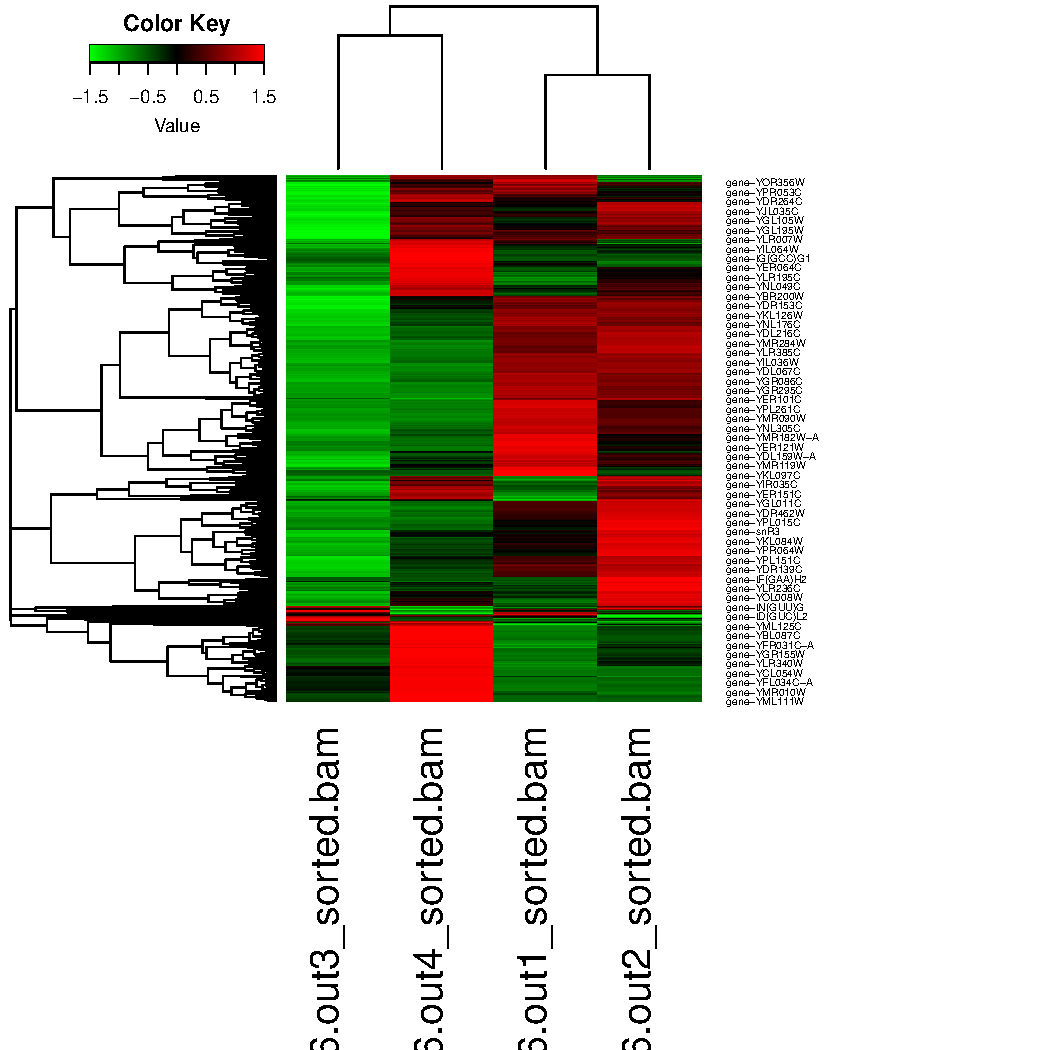
\includepdf[pages=-]{../output.pdf}


\end{document}
